\documentclass[../phys-f308.tex]{subfiles}

\begin{document}
    \part{L1 : Intermolecular forces}
    \begin{abstract}
        In the study of matter, one defines several different states. In this course, we will focus on the study of the properties of condensed matter. Crystals and liquids are examples of such condensed matter - the interaction between molecules of the latter is of the order of $E_{int}>> k_BT$ whereas the former preents an interaction energy $E_{int}\geq k_BT$ which can be put in contrast to a gas' $E_{int}<< k_BT$. Let us note that thermal energy is much larger than the interactions between particules in the gaseous states. 
    \end{abstract}

    \section{Microscopic interaction potential}

    Let us consider the interaction between two different molecules. The total energy in the system can be written as
    \begin{equation}
        E_{tot}(r) = E_A+E_B+w(r)
    \end{equation}
    where $r$ is the distance between the molecules $A$ and $B$ and $w(r)$ is the \emph{potential of interaction}, defined as
    \begin{align}
        w(r) &= E_{tot}(r) - E_{tot}(\infty)\\
        w(r) &= -\int_r^{\infty}F(r)dr \quad \Leftrightarrow \quad F(r) = -\frac{dw}{dr}\label{eq: F dw/dr}
    \end{align}
    Beware to the minus sign between the two: the interaction is \emph{attractive} when the potential is negative, and \emph{repulsive} when the potential   

    \section{Molecular interactions via electrostatic potentials}

    We will perform a review of the electrostatic potential interaction, with an increasing level of complexity. In particular, we will consider the interaction between...
    \begin{itemize}
        \item Two single point charges (approximation for two ions), dipole moments (approximation for two molecules)
        \item A single point charge and a non-rotating dipole moment
        \item Two non rotating dipole moments
        \item A single point charge and a rotating dipole moment
        \item Two rotating dipole moments
    \end{itemize}

    \subsection{Electrostatic interaction between two point charges}
    Let us consider two single points charges $Q_1$ and $Q_2$ separated by a distance $r$. As a reminder, let us note that the electric field of a charge $Q$ at a distance $r$ is given by $E = \frac{Q}{4\pi\epsilon_r\epsilon_0 r^2}$. Therefore, the electric force of charge $Q_1$ on charge $Q_2$ is given by $F=E_1Q_2 = \frac{Q_1Q_2}{4\pi\epsilon_r\epsilon_0 r^2} = \frac{z_1z_2 e^2}{4\pi\epsilon_r\epsilon_0 r^2}$ by introducing the valence numbers $z_i$. We deduce the macroscopic electrostatic potential
    \begin{equation}
        w(r) = -\frac{z_1z_2e^2}{4\pi\epsilon_r\epsilon_0 r}
    \end{equation} 

    \subsubsection{Electrostatic interaction: application to $NaCl$}

    In a vaccum, one finds that $w_{NaCl} = -8.4\ti 10^{-19}J$. However, at room temperature one has that $U_T = k_BT \approx 1.38\ti 10^{-23} J/K \cdot 291 J = 4\ti 10^{-21}J$. Given that \color{red}$w_{NaCl}>200 k_BT$\footnote{Why do we ignore the negative sign?}\color{black}, NaCl is stable at room temperature in a vaccum. However, put it in a medium with high dielectric constant such as water and $w_{NaCl}^{H_2O}(r) \approx 2.5 k_BT$.

    \subsection{Dipole moments}

    Asymetric molecules bounded by covalent bounds often contains dipole moments. One defines the units of $Debye$ for this purpose: take two charges $e$ and $-e$ separated by a distance of one $Angstrum$:
    \begin{equation*}
        \mu = 4.8 D
    \end{equation*}

    \subsubsection{Dipole moment of water}

    \begin{example}
        The molecule of water can be seen as two $OH$ molecules separated by an angle of $104.5°$. Given that $\mu_{OH} = 1.51 D$, we deduce that the dipole moment of water is given by 
        \begin{equation}
            \mu_{H_2O} = 2\cos\left(\frac{H\hat{O}H}{2}\right)\mu_{HO} = 1.85D
        \end{equation}
    \end{example}

    \subsection{Ion-dipole interaction}\label{sec: ion-dipole interaction}

    Instead of looking a two single point charges and a dipole seperately, let us put them together and see what happens as shown in figure \ref{fig: ion-dipole interaction}. The resulting macroscopic electrostatic potential is
    \begin{equation}
        w(r) = -\frac{qQ}{4\pi\epsilon_0r_A}+\frac{qQ}{4\pi\epsilon_0r_B} = \frac{qQ}{4\pi\epsilon_0}\left(\frac{1}{r_B}-\frac{1}{r_A}\right)\label{eq: ion-dipole interaction 1}
    \end{equation}

    Let us note that $r_A \approx r-\frac{l}{2}\cos\theta$ whereas $r_B\approx r+\frac{l}{2}\cos\theta$. Applying the approximation $\frac{r_A-r_B}{r_Ar_B}\approx -\frac{l\cos\theta}{r^2}$, one finds that  \eqref{eq: ion-dipole interaction 1} can be rewritten as
    
    \begin{equation}
        w(r) \approx -\frac{qQ}{4\pi\epsilon_0}\frac{l\cos\theta}{r^2} = -\mu\frac{Q\cos\theta}{4\pi\epsilon_0r^2} \quad w(r) = -\mu E(r)\cos\theta
    \end{equation}

    The potential is either attractive or repulsive, depending on the orientation of the molecule.

    \begin{figure}[H]
        \centering
        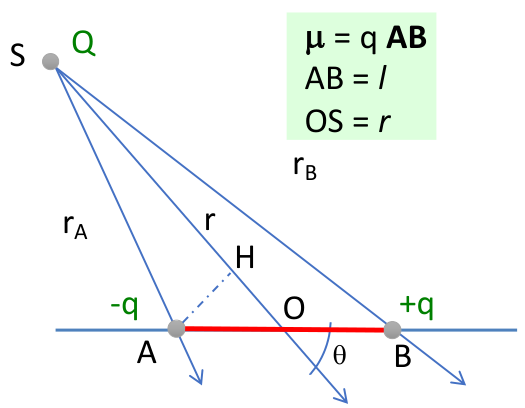
\includegraphics[width=50mm]{partA/Pictures/DipoleIon.png}
        \caption{Ion-dipole interaction}
        \label{fig: ion-dipole interaction}
    \end{figure}

    \subsection{Dipole-dipole interaction}\label{sec: DDipole interaction}

    Assuming the two dipoles can freely move in the $xyz$ space, one would need to replace the angle $\theta$ used previously by three different angles - $\theta_1,\theta_2$ and $\varphi$ as shown in figure \ref{fig: DDipole}. The interaction potential can then be written as
    \begin{equation}
        w(r,\theta_1,\theta_2,\varphi) = -\frac{\mu_1\mu_2}{4\pi\epsilon_o\epsilon_r r^3}\left(2\cos\theta_1\cos\theta_2-\sin\theta_1\sin\theta_2\cos\varphi\right)
    \end{equation}

    To simplify the problem, let us assume the angles $\theta_1$ is equal to $0$, meaning that the only allowed variation is in $\theta_2$ and in the rotation angle $\varphi$. Then,
    \begin{itemize}
        \item $\theta_2 = 0 \quad \Leftrightarrow \quad w(r,0,0,\varphi) = -\frac{2\mu_1\mu_2}{4\pi\epsilon_r\epsilon_0 r^3}$. The two dipoles are attracted to each other.
        \item $\theta_2 = 90$. The dipoles are neither attracted nor repulsed by each other - they are said to be neutral. 
        \item $\theta_2 = 180$. The dipoles are repelled by each other. 
        \item $\theta_2 = 270$. The dipoles are neither attracted nor repulsed by each other - they are said to be neutral.
    \end{itemize}
        Let us note that in all situations, if the dipoles are free to rotate, then they tend to align themselves (situation with the lowest potential). This is shown in figure \ref{dif: DDipole theta1 = 0}.
    
    \begin{figure}[H]
        \begin{subfigure}{.5\textwidth}
            \centering
            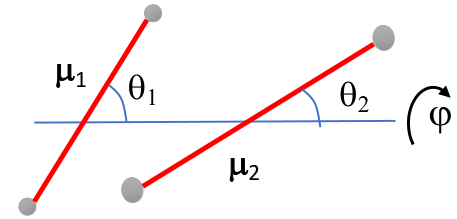
\includegraphics[width=50mm]{partA/Pictures/DDipole.png}
            \caption{Dipole-Dipole interaction}
            \label{fig: DDipole}
        \end{subfigure}
        \begin{subfigure}{.5\textwidth}
            \centering
            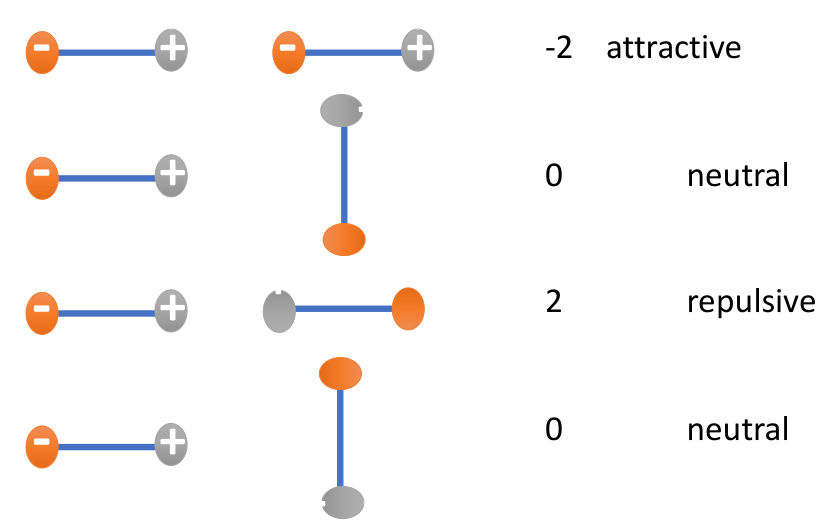
\includegraphics[width=50mm]{partA/Pictures/DDipole_interactions.png}
            \caption{Summary of the different possible states with $\theta_1 = 0$.}
            \label{dif: DDipole theta1 = 0}
        \end{subfigure}
    \end{figure}

    \subsection{Interactions involving freely rotating molecules}

    To take into account all different orientations, one would need to average the potential over the solid angle. Unfortunately, that is difficult to obtain analytically. How can we appropriately approximate the consequences of all the angles? Let us average all the possible orientations over the solid angle $\Omega$.

    \begin{equation}
        e^{-\frac{w(r)}{kT}} = \frac{\int e^{-\frac{w(r,\Omega)}{kT}}d\Omega}{\int d\Omega} = \Bigg\langle e^{-\frac{w(r,\Omega)}{kT}}\Bigg\rangle
    \end{equation}

    When $kT>>w(r,\Omega)$, one finds
    \begin{equation}
        \Bigg\langle\exp\left[-\frac{w(r,\Omega)}{kT}\right]\Bigg\rangle = \Bigg\langle 1 - \frac{w(r,\Omega)}{kT} + \frac{1}{2}\left[\frac{w(r,\Omega)}{kT}\right]^2 + (...)\Bigg\rangle
    \end{equation}

    As the potential is expanded over a Taylor series, it looses its angular contribution and acquires a temperature dependance which leads to
    \begin{equation}
        \overline{w}(r,T) \approx \Bigg\langle w(r,\Omega)-\frac{w(r,\Omega)^2}{2kT}+(...)\Bigg\rangle
    \end{equation}

    \subsubsection{Interaction between a charge and a flexible dipole}

    Reminding ourselves that $\Big\langle\sin\theta\Big\rangle = 0 = \Big\langle\cos\theta\Big\rangle$, and noting that
    \begin{align}
        \int d\Omega &= \int_0^{2\pi}d\phi\int_0^\pi\sin\theta d\theta = 4\pi,\\
        \big\langle\cos^2\theta\big\rangle &= \frac{1}{4\pi} \int_0^\pi \cos^2\theta\sin\theta d\theta\int_0^{2\pi}d\phi = \frac{1}{3},
    \end{align}

    one shows that
    \begin{equation}
        \overline{w}(r,T) \approx \Big\langle-\frac{Q\mu}{4\pi\epsilon_0\epsilon_r r^2}\cos\theta - \left(\frac{Q\mu}{4\pi\epsilon_0\epsilon_r r^2}\right)^2\frac{\cos^2\theta}{2kT} + (...)\Big\rangle = -\frac{Q\mu}{4\pi\epsilon_0\epsilon_r r^2}\big\langle\cos\theta\big\rangle - \frac{1}{2kT}\left(\frac{Q\mu}{4\pi\epsilon_0\epsilon_r r^2}\right)^2\Big\langle\cos^2\theta\Big\rangle + \left(...\right)
    \end{equation}
    meaning that in the limit $kT>>w(r,\Omega)$,
    \begin{equation}
        \overline{w}(r,T) \approx -\frac{1}{6kT}\frac{\left(Q\mu\right)^2}{\left(4\pi\epsilon_0\epsilon_r\right)^2r^4}.
    \end{equation}

    \subsubsection{Interaction between two freely rotating molecules}

    Using the results of \ref{sec: DDipole interaction}, one finds at the high temperature limit $kT>\frac{\mu_1\mu_2}{4\pi\epsilon_0\epsilon_r r^3}$ the expression of the \emph{Keesom forces} (1921)
    \begin{equation}
        \overline{w}(r,T)\approx -\frac{1}{3kT}\frac{\mu_1^2\mu_2^2}{\left(4\pi\epsilon_r\epsilon_0\right)^2}\frac{1}{r^6}\label{eq: Keesom forces}
    \end{equation}

    \subsubsection{Interactions between a charge and a nonpolar molecule}

    The proximity of an ion induces a dipole moment in the nonpolar molecule to appear. If $\Delta E$ is the difference in the electric field induced within the molecule, the magnitude of the dipole acting on the nonpolar molecule is
    \begin{equation}
        E = \mu\frac{\sqrt[]{1+3\cos^2\theta}}{4\pi\epsilon_0\epsilon_r r^3}\label{eq: induced dipole moment}
    \end{equation}
    The interaction potential can then be written as
    \begin{equation}
        w(r,\theta) = -\int fdr = -\int \alpha_0 EdE = -\frac{1}{2}\alpha_0E^2\label{eq: int potential for induced dipole moment}
    \end{equation}
    where we introduced the polarizability constant $\alpha_0 = \frac{\mu}{E}$. Merging \eqref{eq: induced dipole moment} and \eqref{eq: int potential for induced dipole moment}, one finds
    \begin{equation}
        w(r,\theta) = -\frac{\alpha_0\mu^2}{2}\frac{1+3\cos^2\theta}{\left(4\pi\epsilon_0\epsilon_r\right)^2 r^6}
    \end{equation}
    which can be averaged over $\theta$. The interaction between the different molecules is then given by
    \begin{equation}
        w(r) = -\frac{\alpha_{01}\mu_1^2+\alpha_{02}\mu_2^2}{\left(4\pi\epsilon_0\epsilon_r\right)^2r^6}\label{eq: Debye forces}
    \end{equation}
    This is the expression of the \emph{Debye forces} (1920's).

    \subsubsection{Interactions between neutral particules}

    \color{purple}Quantum\color{black}  fluctuations of the charge density inside a nonpolar molecule can induce the formation of an instantaneous dipole moment. This permits interactions with other nonpolar molecules - it is an induced dipole moment. London derived the interaction between $s-electrons$ of two neighboring atoms and solved the problem considering quantum oscillator of frequency $\nu$ and thus of ionization potential $I = h\nu$. The \emph{London (dissipative) forces} (1937) can be written as
    \begin{equation}
        w(r) \approx -\frac{1}{2\left(4\pi\epsilon_0\epsilon_r\right)^2}\frac{\alpha_1\alpha_2}{r^6}\frac{I_1I_2}{I_1+I_2}\label{eq: London (dissipative) forces}
    \end{equation}

    \subsubsection{Van der Waals interactions}

    The Van der Waals forces are comprised of three terms, corresponding to \eqref{eq: Keesom forces} (dipole-dipole),\eqref{eq: Debye forces} (dipole-induced dipole) and \eqref{eq: London (dissipative) forces} (induced dipole-induced dipole). The largest contribution is given by London (20-99\%) and Keesom forces.

    \part{L2: Phase transitions I : Thermodynamics}

\end{document}